\begin{frame}{Phân bố phần cứng trên 5 tầng Pipeline}
    Đường truyền dữ liệu (Datapath) ánh xạ trực tiếp các module Verilog vào từng giai đoạn xử lý:
    \vspace{0.3cm}
    
    \centering
    \begin{tikzpicture}[
        stage/.style={draw=DeepBlue, fill=DeepBlue!6, minimum width=1.8cm, minimum height=1.2cm, rounded corners=4pt, line width=1.2pt, font=\scriptsize, text width=1.75cm, align=center},
        reg/.style={draw=AccentGreen!80!black, fill=AccentGreen!12, minimum width=0.4cm, minimum height=1.8cm, rounded corners=1.5pt, line width=1.2pt, font=\tiny\bfseries\color{DeepBlue!90!black}, align=center},
        arrow/.style={->, >=stealth, line width=1.5pt, DeepBlue!85}
    ]
        % Stages & Registers
        \node[stage] (if) at (0.9, 0) {\textbf{Fetch (IF)}\\[0.05cm]\tiny\color{black!70}\texttt{pc\_logic}\\[0.02cm]\tiny\color{black!70}\texttt{instr\_mem}};
        \node[reg] (ifid) at (2.3, 0) {\makebox[0pt][c]{\rotatebox{90}{IF/ID}}};
        
        \node[stage] (id) at (3.7, 0) {\textbf{Decode (ID)}\\[0.05cm]\tiny\color{black!70}\texttt{control\_unit}\\[0.02cm]\tiny\color{black!70}\texttt{reg\_file}};
        \node[reg] (idex) at (5.1, 0) {\makebox[0pt][c]{\rotatebox{90}{ID/EX}}};
        
        \node[stage] (ex) at (6.5, 0) {\textbf{Execute (EX)}\\[0.05cm]\tiny\color{black!70}\texttt{alu}};
        \node[reg] (exmem) at (7.9, 0) {\makebox[0pt][c]{\rotatebox{90}{EX/MEM}}};
        
        \node[stage] (mem) at (9.3, 0) {\textbf{Memory (MEM)}\\[0.05cm]\tiny\color{black!70}Liên kết\\[0.02cm]\tiny\color{black!70}\texttt{data\_mem}};
        \node[reg] (memwb) at (10.7, 0) {\makebox[0pt][c]{\rotatebox{90}{MEM/WB}}};
        
        \node[stage] (wb) at (12.1, 0) {\textbf{Writeback (WB)}\\[0.05cm]\tiny\color{black!70}Ghi tập\\[0.02cm]\tiny\color{black!70}thanh ghi};
        
        % Clock triangles at the bottom of pipeline registers
        \draw[line width=1.2pt, AccentGreen!80!black] (2.2, -0.9) -- (2.3, -0.78) -- (2.4, -0.9);
        \draw[line width=1.2pt, AccentGreen!80!black] (5.0, -0.9) -- (5.1, -0.78) -- (5.2, -0.9);
        \draw[line width=1.2pt, AccentGreen!80!black] (7.8, -0.9) -- (7.9, -0.78) -- (8.0, -0.9);
        \draw[line width=1.2pt, AccentGreen!80!black] (10.6, -0.9) -- (10.7, -0.78) -- (10.8, -0.9);
        
        % Connections
        \draw[arrow] (if.east) -- (ifid.west);
        \draw[arrow] (ifid.east) -- (id.west);
        \draw[arrow] (id.east) -- (idex.west);
        \draw[arrow] (idex.east) -- (ex.west);
        \draw[arrow] (ex.east) -- (exmem.west);
        \draw[arrow] (exmem.east) -- (mem.west);
        \draw[arrow] (mem.east) -- (memwb.west);
        \draw[arrow] (memwb.east) -- (wb.west);
    \end{tikzpicture}
    
    \vspace{0.3cm}
    \begin{block}{Nguyên lý hoạt động của Đường dữ liệu}
        \scriptsize
        \begin{itemize}
            \item \textbf{Khối logic chức năng} (\texttt{pc\_logic}, \texttt{reg\_file}, \texttt{alu},...) thực hiện nhiệm vụ xử lý trong từng tầng riêng biệt.
            \item \textbf{Thanh ghi đệm Pipeline} (\texttt{IF/ID}, \texttt{ID/EX},...) đóng vai trò chốt dữ liệu giữa các sườn clock, giữ cho lệnh ở các tầng không bị trộn lẫn khi thực thi song song.
        \end{itemize}
    \end{block}
\end{frame}

\subsection{Các khối xử lý logic chức năng}
\subsubsection{Bộ nhớ lệnh (Instruction Memory)}
\begin{frame}[fragile]{Bộ nhớ lệnh (\texttt{instr\_mem.v})}
    \begin{columns}
        \begin{column}{0.48\textwidth}
            \centering
            \textbf{Sơ đồ khối chức năng}
            \vspace{0.3cm}
            
            \begin{tikzpicture}[
                block/.style={draw, thick, fill=blue!10, draw=DeepBlue, minimum width=3.2cm, minimum height=1.8cm, rounded corners, font=\scriptsize\bfseries, align=center},
                bus/.style={->, >=stealth, double, double distance=1.5pt, thick, DeepBlue}
            ]
                % Main Memory Block
                \node[block] (mem) at (0, 0) {Instruction Memory\\[0.15cm]\tiny (\texttt{instr\_mem.v})\\[0.2cm]\scriptsize Mảng nhớ: 256 $\times$ 32-bit};
                
                % Inputs
                \draw[bus] (-2.6, 0) -- node[above=0.05cm, font=\tiny\bfseries] {addr[31:0]} (mem.west);
                
                % Outputs
                \draw[bus] (mem.east) -- node[above=0.05cm, font=\tiny\bfseries] {instruction[31:0]} (2.6, 0);
            \end{tikzpicture}
        \end{column}
        
        \begin{column}{0.48\textwidth}
            \begin{block}{Mã nguồn Verilog đầy đủ}
                \begin{lstlisting}[language=Verilog, basicstyle=\tiny\ttfamily, keywordstyle=\color{blue}, commentstyle=\color{gray}]
module instr_mem #(
    parameter INIT_FILE = "program.hex",
    parameter PROGRAM_WORDS = 256
)(
    input  wire [31:0] addr,
    output wire [31:0] instruction
);
    reg [31:0] mem [0:255];
    wire [7:0] word_addr = addr[9:2];

    assign instruction = mem[word_addr];

    integer i;
    initial begin
        // Khoi tao NOP truoc khi nap
        for (i = 0; i < 256; i = i + 1)
            mem[i] = 32'h0000_0013;
        $readmemh(INIT_FILE, mem, 0, PROGRAM_WORDS - 1);
    end
endmodule
                \end{lstlisting}
            \end{block}
        \end{column}
    \end{columns}
\end{frame}
\subsubsection{Khối PC Logic}
\begin{frame}[fragile]{PC Logic: Sơ đồ \& Nguyên lý hoạt động}
    \begin{columns}
        \begin{column}{0.48\textwidth}
            \centering
            \textbf{Sơ đồ khối chức năng}
            \vspace{0.2cm}
            
            \begin{tikzpicture}[
                block/.style={draw, thick, fill=blue!10, draw=DeepBlue, minimum width=3.0cm, minimum height=2.8cm, rounded corners, font=\scriptsize\bfseries, align=center},
                bus/.style={->, >=stealth, double, double distance=1.5pt, thick, DeepBlue},
                wire/.style={->, >=stealth, thick, DeepBlue}
            ]
                % Main Block
                \node[block] (pc_block) at (0, 0) {PC Logic\\[0.15cm]\tiny (\texttt{pc\_logic.v})};
                
                % Inputs (Left side)
                \draw[wire] (-2.2, 1.05) -- node[above, font=\tiny\bfseries] {clk} ([yshift=1.05cm]pc_block.west);
                \draw[wire] (-2.2, 0.70) -- node[above, font=\tiny\bfseries] {reset} ([yshift=0.70cm]pc_block.west);
                \draw[wire] (-2.2, 0.35) -- node[above, font=\tiny\bfseries] {stall} ([yshift=0.35cm]pc_block.west);
                
                \draw[wire] (-2.2, -0.15) -- node[above, font=\tiny\bfseries] {branch\_taken} ([yshift=-0.15cm]pc_block.west);
                \draw[bus] (-2.2, -0.50) -- node[above=0.02cm, font=\tiny\bfseries] {branch\_target} ([yshift=-0.50cm]pc_block.west);
                
                \draw[wire] (-2.2, -0.85) -- node[above, font=\tiny\bfseries] {jump} ([yshift=-0.85cm]pc_block.west);
                \draw[bus] (-2.2, -1.20) -- node[above=0.02cm, font=\tiny\bfseries] {jump\_target} ([yshift=-1.20cm]pc_block.west);
                
                % Outputs (Right side)
                \draw[bus] (pc_block.east) -- node[above=0.05cm, font=\tiny\bfseries] {pc[31:0]} (2.2, 0);
            \end{tikzpicture}
        \end{column}
        
        \begin{column}{0.48\textwidth}
            \begin{block}{Nguyên lý cập nhật địa chỉ PC}
                \scriptsize
                Quy trình cập nhật PC theo mức độ ưu tiên giảm dần:
                \begin{enumerate}
                    \item \textbf{Reset:} Đưa địa chỉ PC về 0 khi bắt đầu.
                    \item \textbf{Stall:} Đóng băng PC (giữ nguyên giá trị cũ) khi gặp xung đột dữ liệu hoặc tài nguyên.
                    \item \textbf{Jump:} Nhập địa chỉ nhảy không điều kiện (`jump\_target`) từ các lệnh `JAL`, `JALR`.
                    \item \textbf{Branch:} Nhập địa chỉ rẽ nhánh (`branch\_target`) khi điều kiện rẽ nhánh thỏa mãn (\texttt{branch\_taken} = 1).
                \end{enumerate}
            \end{block}
        \end{column}
    \end{columns}
\end{frame}

\begin{frame}[fragile]{PC Logic: Hiện thực mã nguồn Verilog}
    \begin{columns}[t]
        \begin{column}{0.46\textwidth}
            \begin{block}{Khai báo Module \& Ports}
                \begin{lstlisting}[language=Verilog, basicstyle=\fontsize{6.5pt}{8.0pt}\selectfont\ttfamily, keywordstyle=\color{blue}, commentstyle=\color{gray}]
module pc_logic (
    input  wire        clk,
    input  wire        reset,
    input  wire        stall,

    input  wire        branch_taken,
    input  wire [31:0] branch_target,

    input  wire        jump,
    input  wire [31:0] jump_target,

    output reg  [31:0] pc
);
                \end{lstlisting}
            \end{block}
        \end{column}
        
        \begin{column}{0.50\textwidth}
            \begin{block}{Khối Logic Cập Nhật PC}
                \begin{lstlisting}[language=Verilog, basicstyle=\fontsize{6.5pt}{8.0pt}\selectfont\ttfamily, keywordstyle=\color{blue}, commentstyle=\color{gray}]
    always @(posedge clk or posedge reset) begin
        if (reset) begin
            pc <= 32'd0;
        end
        else if (stall) begin
            pc <= pc;
        end
        else if (jump) begin
            pc <= jump_target;
        end
        else if (branch_taken) begin
            pc <= branch_target;
        end
        else begin
            pc <= pc + 32'd4;
        end
    end

endmodule
                \end{lstlisting}
            \end{block}
        \end{column}
    \end{columns}
\end{frame}

\begin{frame}[fragile]{PC Logic: Thiết lập môi trường Testbench}
    \begin{columns}[t]
        \begin{column}{0.46\textwidth}
            \begin{block}{Khai báo Tín hiệu \& Mạch nạp}
                \begin{lstlisting}[language=Verilog, basicstyle=\fontsize{6.5pt}{8.0pt}\selectfont\ttfamily, keywordstyle=\color{blue}, commentstyle=\color{gray}]
`timescale 1ns/1ps

module pc_logic_tb;

    reg clk;
    reg reset;
    reg stall;

    reg branch_taken;
    reg [31:0] branch_target;

    reg jump;
    reg [31:0] jump_target;

    wire [31:0] pc;
                \end{lstlisting}
            \end{block}
        \end{column}
        
        \begin{column}{0.50\textwidth}
            \begin{block}{Khởi tạo UUT \& Bộ tạo Xung nhịp}
                \begin{lstlisting}[language=Verilog, basicstyle=\fontsize{6.5pt}{7.5pt}\selectfont\ttfamily, keywordstyle=\color{blue}, commentstyle=\color{gray}]
    pc_logic uut (
        .clk(clk),
        .reset(reset),
        .stall(stall),
        .branch_taken(branch_taken),
        .branch_target(branch_target),
        .jump(jump),
        .jump_target(jump_target),
        .pc(pc)
    );

    always #5 clk = ~clk;
                \end{lstlisting}
            \end{block}
        \end{column}
    \end{columns}
\end{frame}

\begin{frame}[fragile]{PC Logic: Kịch bản kiểm thử}
    \begin{columns}[t]
        \begin{column}{0.48\textwidth}
            \begin{block}{Kịch bản kích thích chính}
                \begin{lstlisting}[language=Verilog, basicstyle=\fontsize{6.5pt}{8.0pt}\selectfont\ttfamily, keywordstyle=\color{blue}, commentstyle=\color{gray}]
    initial begin
        clk = 0; reset = 1; stall = 0;
        branch_taken = 0; branch_target = 0;
        jump = 0; jump_target = 0;
        #10 reset = 0;
        #20; // Normal PC increment
        stall = 1; #10; stall = 0; // Stall
        branch_taken = 1; branch_target = 100;
        #10; branch_taken = 0; // Branch
        jump = 1; jump_target = 200;
        #10; jump = 0; // Jump
        #20; $finish;
    end
                \end{lstlisting}
            \end{block}
        \end{column}
        
        \begin{column}{0.48\textwidth}
            \begin{block}{Giám sát tín hiệu \& Lưu dạng sóng}
                \begin{lstlisting}[language=Verilog, basicstyle=\fontsize{6.5pt}{8.0pt}\selectfont\ttfamily, keywordstyle=\color{blue}, commentstyle=\color{gray}]
    initial begin
        $monitor(
            "t=%0t pc=%0d s=%b b=%b j=%b",
            $time, pc, stall, branch_taken, jump
        );
    end

    initial begin
        $dumpfile("pc_logic_tb.vcd");
        $dumpvars(0, pc_logic_tb);
    end

endmodule
                \end{lstlisting}
            \end{block}
        \end{column}
    \end{columns}
\end{frame}
\begin{frame}[fragile]{PC Logic: Kết Quả Mô Phỏng Console}
    \begin{columns}
        \begin{column}{0.55\textwidth}
            \begin{block}{Console Output (\$monitor)}
                \begin{lstlisting}[basicstyle=\fontsize{7.5pt}{9.0pt}\selectfont\ttfamily, numbers=none]
Time=0 | PC=         0 | stall=0 | branch=0 | jump=0
Time=15000 | PC=         4 | stall=0 | branch=0 | jump=0
Time=25000 | PC=         8 | stall=0 | branch=0 | jump=0
Time=30000 | PC=         8 | stall=1 | branch=0 | jump=0
Time=40000 | PC=         8 | stall=0 | branch=1 | jump=0
Time=45000 | PC=       100 | stall=0 | branch=1 | jump=0
Time=50000 | PC=       100 | stall=0 | branch=0 | jump=1
Time=55000 | PC=       200 | stall=0 | branch=0 | jump=1
Time=60000 | PC=       200 | stall=0 | branch=0 | jump=0
Time=65000 | PC=       204 | stall=0 | branch=0 | jump=0
Time=75000 | PC=       208 | stall=0 | branch=0 | jump=0
tb/pc_logic_tb.v:63: $finish called at 80000 (1ps)
                \end{lstlisting}
            \end{block}
        \end{column}
        
        \begin{column}{0.41\textwidth}
            \begin{block}{Phân tích kịch bản kiểm thử}
                \scriptsize
                \begin{itemize}
                    \item \textbf{0ns -- 30ns (Tăng tuần tự):} PC tăng tuần tự +4 sau mỗi chu kỳ clock (0 $\rightarrow$ 4 $\rightarrow$ 8).
                    \item \textbf{30ns -- 40ns (Đóng băng):} Tín hiệu \texttt{stall=1}, PC giữ nguyên giá trị bằng 8.
                    \item \textbf{40ns -- 50ns (Rẽ nhánh):} Tín hiệu \texttt{branch\_taken=1}, PC cập nhật địa chỉ nhánh bằng 100.
                    \item \textbf{50ns -- 60ns (Lệnh nhảy):} Tín hiệu \texttt{jump=1}, PC cập nhật địa chỉ nhảy bằng 200.
                \end{itemize}
            \end{block}
        \end{column}
    \end{columns}
\end{frame}

\begin{frame}{PC Logic: Giản Đồ Sóng Mô Phỏng (GTKWave)}
    \begin{block}{Giản đồ sóng chi tiết}
        \centering
        \vspace{0.05cm}
        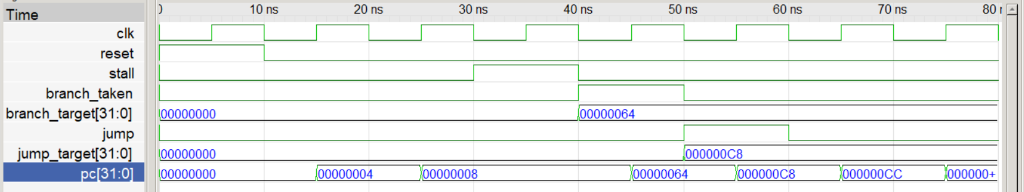
\includegraphics[width=0.98\textwidth]{design/test/pc_test.png}
        \vspace{0.05cm}
    \end{block}
    \vspace{0.1cm}
    \begin{block}{Nhận xét kết quả trên dạng sóng}
        \scriptsize
        \begin{itemize}
            \item \textbf{Thời điểm 30ns (Stall):} Khi \texttt{stall} lên 1, giá trị PC được chốt giữ nguyên ở mức 8 tại sườn lên clock tiếp theo.
            \item \textbf{Thời điểm 40ns (Branch):} Địa chỉ rẽ nhánh \texttt{branch\_target} = \texttt{0x00000064} (100) được nạp thành công vào PC.
            \item \textbf{Thời điểm 50ns (Jump):} Địa chỉ nhảy \texttt{jump\_target} = \texttt{0x000000C8} (200) được cập nhật thành công vào PC.
        \end{itemize}
    \end{block}
\end{frame}
\subsubsection{Khối Tập thanh ghi (Register File)}
\begin{frame}[fragile]{Khối Tập Thanh Ghi (\texttt{reg\_file.v})}
    \begin{columns}
        \begin{column}{0.46\textwidth}
            \centering
            \textbf{Sơ đồ khối chức năng}
            \vspace{0.2cm}
            
            \begin{tikzpicture}[
                block/.style={draw, thick, fill=blue!10, draw=DeepBlue, minimum width=2.8cm, minimum height=2.6cm, rounded corners, font=\scriptsize\bfseries, align=center},
                bus/.style={->, >=stealth, double, double distance=1.5pt, thick, DeepBlue},
                wire/.style={->, >=stealth, thick, DeepBlue}
            ]
                % Main Block
                \node[block] (rf) at (0, 0) {Register File\\[0.1cm]\tiny (\texttt{reg\_file.v})};
                
                % Inputs (Left side)
                \draw[wire] (-2.0, 0.9) -- node[above, font=\tiny\bfseries] {clk} ([yshift=0.9cm]rf.west);
                \draw[bus] (-2.0, 0.4) -- node[above=0.01cm, font=\tiny\bfseries] {rs1\_addr} ([yshift=0.4cm]rf.west);
                \draw[bus] (-2.0, 0.0) -- node[above=0.01cm, font=\tiny\bfseries] {rs2\_addr} ([yshift=0.0cm]rf.west);
                \draw[bus] (-2.0, -0.4) -- node[above=0.01cm, font=\tiny\bfseries] {rd\_addr} ([yshift=-0.4cm]rf.west);
                \draw[bus] (-2.0, -0.9) -- node[above=0.01cm, font=\tiny\bfseries] {wdata} ([yshift=-0.9cm]rf.west);
                
                % Control Input (Top side)
                \draw[wire] (0, 1.7) -- node[right, font=\tiny\bfseries] {reg\_write} (rf.north);
                
                % Outputs (Right side)
                \draw[bus] ([yshift=0.4cm]rf.east) -- node[above=0.01cm, font=\tiny\bfseries] {rs1\_data} (2.0, 0.4);
                \draw[bus] ([yshift=-0.4cm]rf.east) -- node[above=0.01cm, font=\tiny\bfseries] {rs2\_data} (2.0, -0.4);
            \end{tikzpicture}
            
            \vspace{0.15cm}
            \scriptsize
            \begin{block}{Nguyên lý hoạt động}
                \begin{itemize}
                    \item \textbf{Quy mô:} 32 thanh ghi 32-bit (x0 cứng về 0).
                    \item \textbf{Đọc bất đồng bộ:} rs1\_data, rs2\_data.
                    \item \textbf{Ghi đồng bộ:} rd khi reg\_write=1.
                    \item \textbf{Cầu bypass:} Tránh trễ 1 chu kỳ khi đọc-ghi cùng thanh ghi.
                \end{itemize}
            \end{block}
        \end{column}
        
        \begin{column}{0.52\textwidth}
            \begin{block}{Mã nguồn Verilog tập thanh ghi}
                \begin{lstlisting}[language=Verilog, basicstyle=\fontsize{6.0pt}{6.8pt}\selectfont\ttfamily, keywordstyle=\color{blue}, commentstyle=\color{gray}]
module reg_file (
    input  wire        clk, reset,
    input  wire [4:0]  rs1_addr, rs2_addr, rd_addr,
    input  wire [31:0] write_data,
    input  wire        reg_write,
    output wire [31:0] rs1_data, rs2_data
);
    reg [31:0] registers [0:31];

    assign rs1_data = (rs1_addr == 5'd0) ? 32'd0 :
                      (reg_write && (rd_addr == rs1_addr)) 
                      ? write_data : registers[rs1_addr];
    assign rs2_data = (rs2_addr == 5'd0) ? 32'd0 :
                      (reg_write && (rd_addr == rs2_addr)) 
                      ? write_data : registers[rs2_addr];

    integer i;
    always @(posedge clk or posedge reset) begin
        if (reset) begin
            for (i = 0; i < 32; i = i + 1)
                registers[i] <= 32'd0;
        end else if (reg_write && (rd_addr != 5'd0)) begin
            registers[rd_addr] <= write_data;
        end
    end
endmodule
                \end{lstlisting}
            \end{block}
        \end{column}
    \end{columns}
\end{frame}

\subsubsection{Khối Tính toán Số học \& Logic (ALU)}
\begin{frame}[fragile]{Khối Tính Toán Số Học \& Logic (\texttt{alu.v})}
    \begin{columns}
        \begin{column}{0.46\textwidth}
            \centering
            \textbf{Sơ đồ khối chức năng}
            \vspace{0.2cm}
            
            \begin{tikzpicture}[
                alu/.style={draw, thick, fill=blue!10, draw=DeepBlue, minimum width=2.4cm, minimum height=1.6cm, font=\scriptsize\bfseries, align=center},
                bus/.style={->, >=stealth, double, double distance=1.5pt, thick, DeepBlue},
                wire/.style={->, >=stealth, thick, DeepBlue}
            ]
                % Main ALU Block
                \node[alu] (alu_block) at (0, 0) {ALU\\[0.15cm]\tiny (\texttt{alu.v})};
                
                % Inputs
                \draw[bus] (-2.2, 0.4) -- node[above=0.01cm, font=\tiny\bfseries] {a[31:0]} ([yshift=0.4cm]alu_block.west);
                \draw[bus] (-2.2, -0.4) -- node[above=0.01cm, font=\tiny\bfseries] {b[31:0]} ([yshift=-0.4cm]alu_block.west);
                \draw[bus] (0, 1.4) -- node[right, font=\tiny\bfseries] {alu\_control[3:0]} (alu_block.north);
                
                % Outputs
                \draw[bus] ([yshift=0.3cm]alu_block.east) -- node[above=0.01cm, font=\tiny\bfseries] {result[31:0]} (2.2, 0.3);
                \draw[wire] ([yshift=-0.3cm]alu_block.east) -- node[above=0.01cm, font=\tiny\bfseries] {zero} (2.2, -0.3);
            \end{tikzpicture}
            
            \vspace{0.2cm}
            \scriptsize
            \begin{block}{Đặc tả hoạt động}
                \begin{itemize}
                    \item \textbf{Phép toán số học:} ADD (cộng), SUB (trừ), so sánh có dấu SLT.
                    \item \textbf{Phép toán logic:} AND, OR, XOR và dịch chuyển bit logic (SLL, SRL).
                    \item \textbf{Cờ Zero:} Tín hiệu ra 1-bit, tích cực mức cao khi kết quả toán học bằng 0 (dùng cho lệnh rẽ nhánh).
                \end{itemize}
            \end{block}
        \end{column}
        
        \begin{column}{0.52\textwidth}
            \begin{block}{Hiện thực khối Case ALU}
                \begin{lstlisting}[language=Verilog, basicstyle=\fontsize{6.0pt}{7.2pt}\selectfont\ttfamily, keywordstyle=\color{blue}, commentstyle=\color{gray}]
always @(*) begin
    case (alu_control)
        4'b0010: result = a + b; // ADD
        4'b0110: result = a - b; // SUB
        4'b0000: result = a & b; // AND
        4'b0001: result = a | b; // OR
        4'b0100: result = a ^ b; // XOR
        4'b0011: result = a << b[4:0]; // SLL
        4'b0101: result = a >> b[4:0]; // SRL
        4'b0111: result = ($signed(a) < $signed(b)) 
                          ? 32'd1 : 32'd0; // SLT
        default: result = 32'b0;
    endcase
end

// Co bao Zero
assign zero = (result == 32'b0);
                \end{lstlisting}
            \end{block}
        \end{column}
    \end{columns}
\end{frame}

\begin{frame}[fragile]{ALU: Kịch bản kiểm thử (Testbench)}
    \begin{columns}[t]
        \begin{column}{0.48\textwidth}
            \begin{block}{DUT \& Khai báo tín hiệu}
                \begin{lstlisting}[language=Verilog, basicstyle=\fontsize{6.0pt}{7.0pt}\selectfont\ttfamily, keywordstyle=\color{blue}, commentstyle=\color{gray}]
module alu_tb();
    reg  [31:0] a, b;
    reg  [3:0]  alu_control;
    wire [31:0] result;
    wire        zero;

    // Khoi tao Device Under Test (DUT)
    alu dut (
        .a(a), .b(b),
        .alu_control(alu_control),
        .result(result), .zero(zero)
    );

    localparam AND  = 4'b0000;
    localparam OR   = 4'b0001;
    localparam ADD  = 4'b0010;
    localparam SLL  = 4'b0011;
    localparam XOR  = 4'b0100;
    localparam SRL  = 4'b0101;
    localparam SUB  = 4'b0110;
    localparam SLT  = 4'b0111;
                \end{lstlisting}
            \end{block}
        \end{column}
        
        \begin{column}{0.48\textwidth}
            \begin{block}{Kịch bản kích thích chính}
                \begin{lstlisting}[language=Verilog, basicstyle=\fontsize{6.0pt}{7.0pt}\selectfont\ttfamily, keywordstyle=\color{blue}, commentstyle=\color{gray}]
    initial begin
        $dumpfile("tb/alu_tb.vcd");
        $dumpvars(0, alu_tb);
        // Cases: ADD, SUB, AND, SLT (pos/neg)
        a = 10; b = 20; alu_control = ADD; #10;
        a = 50; b = 50; alu_control = SUB; #10;
        a = 32'hAAAA_AAAA; b = 32'h5555_5555; 
        alu_control = AND; #10;
        a = 15; b = 25; alu_control = SLT; #10;
        a = -10; b = 5; alu_control = SLT; #10;
        // Cases: OR, XOR, SLL, SRL
        a = 32'hF0F0_FFFF; b = 32'h0F0F_0000; 
        alu_control = OR; #10;
        a = 32'hF0F0_FFFF; b = 32'hFFFF_0000; 
        alu_control = XOR; #10;
        a = 32'h0000_000F; b = 4; alu_control = SLL; #10;
        a = 32'hF000_0000; b = 4; alu_control = SRL; #10;
        $finish;
    end
                \end{lstlisting}
            \end{block}
        \end{column}
    \end{columns}
\end{frame}

\begin{frame}[fragile]{ALU: Kết quả mô phỏng Console}
    Mô phỏng thực thi chính xác toàn bộ 9 kịch bản kiểm thử trên Console:
    \vspace{0.1cm}
    
    \begin{block}{Kết quả xuất ra màn hình (Console Output)}
        \begin{lstlisting}[basicstyle=\fontsize{5.5pt}{6.5pt}\selectfont\ttfamily]
Time |     A (Hex) [Dec]     |     B (Hex) [Dec]     | Control |   Result [Dec]    | Zero
-----|-----------------------|-----------------------|---------|-------------------|-----
  10 | 0x0000000a (  10)     | 0x00000014 (  20)     |   ADD   | 0x0000001e (  30) |  0
  20 | 0x00000032 (  50)     | 0x00000032 (  50)     |   SUB   | 0x00000000 (   0) |  1
  30 | 0xaaaaaaaa (-1.43G)   | 0x55555555 ( 1.43G)   |   AND   | 0x00000000 (   0) |  1
  40 | 0x0000000f (  15)     | 0x00000019 (  25)     |   SLT   | 0x00000001 (   1) |  0
  50 | 0xfffffff6 ( -10)     | 0x00000005 (   5)     |   SLT   | 0x00000001 (   1) |  0
  60 | 0xf0f0ffff (-252M)    | 0x0f0f0000 ( 252M)    |   OR    | 0xffffffff (  -1) |  0
  70 | 0xf0f0ffff (-252M)    | 0xffff0000 ( -65K)    |   XOR   | 0x0f0fffff ( 252M)|  0
  80 | 0x0000000f (  15)     | 0x00000004 (   4)     |   SLL   | 0x000000f0 ( 240) |  0
  90 | 0xf0000000 (-268M)    | 0x00000004 (   4)     |   SRL   | 0x0f000000 ( 251M)|  0
-----|-----------------------|-----------------------|---------|-------------------|-----
Kiem tra ket thuc.
        \end{lstlisting}
    \end{block}
    
    \vspace{-0.05cm}
    \scriptsize
    \textbf{Nhận xét kết quả:}
    \begin{itemize}
        \item \textbf{Phép toán số học \& logic:} Cộng (`ADD`), trừ (`SUB`), `AND`, `OR`, `XOR` cho kết quả chính xác 100\%.
        \item \textbf{So sánh có dấu SLT:} Kiểm chứng đúng cho cả số dương và số âm ($-10 < 5$ ra kết quả bằng `1`).
        \item \textbf{Dịch chuyển bit SLL/SRL:} Dịch chuyển đúng số bit được yêu cầu (ví dụ: dịch trái `0xF` đi 4 bit ra `0xF0`).
        \item \textbf{Cờ Zero:} Tự động phản hồi lên `1` khi kết quả tính toán bằng 0 (như ở phép `SUB` và `AND`).
    \end{itemize}
\end{frame}

\begin{frame}{ALU: Giản Đồ Sóng Mô Phỏng (GTKWave)}
    \begin{block}{Giản đồ sóng chi tiết thu được từ bộ mô phỏng}
        \centering
        \vspace{0.05cm}
        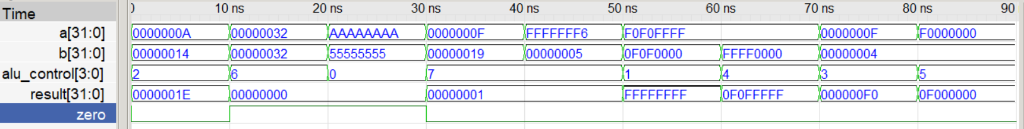
\includegraphics[width=0.95\textwidth]{design/test/alu_test.png}
        \vspace{0.05cm}
    \end{block}
    \vspace{0.15cm}
    \begin{columns}[t]
        \begin{column}{0.48\textwidth}
            \small\textbf{\color{DeepBlue}$\bullet$ Tín hiệu ngõ vào (Inputs)}
            \vspace{0.05cm}
            \scriptsize
            \begin{itemize}
                \item \texttt{a[31:0]}, \texttt{b[31:0]}: Toán hạng ngõ vào (dạng Hex).
                \item \texttt{alu\_control[3:0]}: Mã lệnh điều khiển (\texttt{2}=ADD, \texttt{6}=SUB, \texttt{0}=AND, \texttt{7}=SLT, \texttt{1}=OR, \texttt{4}=XOR, \texttt{3}=SLL, \texttt{5}=SRL).
            \end{itemize}
        \end{column}
        
        \begin{column}{0.48\textwidth}
            \small\textbf{\color{DeepBlue}$\bullet$ Tín hiệu ngõ ra (Outputs)}
            \vspace{0.05cm}
            \scriptsize
            \begin{itemize}
                \item \texttt{result[31:0]}: Kết quả tính toán (dạng Hex).
                \item \texttt{zero}: Cờ báo bằng không, mức cao (\texttt{1}) khi \texttt{result} = 0.
            \end{itemize}
        \end{column}
    \end{columns}
\end{frame}


\subsubsection{Bộ nhớ dữ liệu (Data Memory)}
\begin{frame}[fragile]{Bộ Nhớ Dữ Liệu Dùng Chung (\texttt{data\_mem.v})}
    \begin{columns}
        \begin{column}{0.46\textwidth}
            \centering
            \textbf{Sơ đồ khối chức năng}
            \vspace{0.2cm}
            
            \begin{tikzpicture}[
                block/.style={draw, thick, fill=blue!10, draw=DeepBlue, minimum width=3.0cm, minimum height=2.4cm, rounded corners, font=\scriptsize\bfseries, align=center},
                bus/.style={->, >=stealth, double, double distance=1.5pt, thick, DeepBlue},
                ctrl/.style={->, >=stealth, thick, red!70!black}
            ]
                % Main Block
                \node[block] (mem) at (0, 0) {Shared RAM 4KB\\[0.1cm]\tiny (\texttt{data\_mem.v})};
                
                % Control Inputs (Left side - Red lines)
                \draw[ctrl] (-2.2, 0.9) -- node[above, font=\tiny\bfseries] {clk} ([yshift=0.9cm]mem.west);
                \draw[ctrl] (-2.2, 0.6) -- node[above, font=\tiny\bfseries] {reset} ([yshift=0.6cm]mem.west);
                \draw[ctrl] (-2.2, 0.3) -- node[above, font=\tiny\bfseries] {we} ([yshift=0.3cm]mem.west);
                \draw[ctrl] (-2.2, 0.0) -- node[above, font=\tiny\bfseries] {re} ([yshift=0.0cm]mem.west);
                
                % Data/Address Inputs (Left side - Double Blue lines)
                \draw[bus] (-2.2, -0.4) -- node[above=0.01cm, font=\tiny\bfseries] {addr[31:0]} ([yshift=-0.4cm]mem.west);
                \draw[bus] (-2.2, -0.8) -- node[above=0.01cm, font=\tiny\bfseries] {wdata[31:0]} ([yshift=-0.8cm]mem.west);
                
                % Data Outputs (Right side - Double Blue line)
                \draw[bus] (mem.east) -- node[above=0.01cm, font=\tiny\bfseries] {rdata[31:0]} (2.2, 0);
            \end{tikzpicture}
            
            \vspace{0.2cm}
            \scriptsize
            \begin{block}{Cơ chế hoạt động bộ nhớ}
                \begin{itemize}
                    \item \textbf{Căn lề địa chỉ (Word-aligned):} Lấy 10 bit địa chỉ thực tế \texttt{addr[11:2]} để lập chỉ mục 1024 từ nhớ (mỗi từ 32-bit).
                    \item \textbf{Đọc tổ hợp (Bất đồng bộ):} Trả về rdata lập tức khi đổi địa chỉ và re=1 (thuận tiện cho kết nối Bus).
                    \item \textbf{Ghi đồng bộ:} Cập nhật mảng nhớ tại cạnh lên clk khi we=1.
                \end{itemize}
            \end{block}
        \end{column}
        
        \begin{column}{0.52\textwidth}
            \begin{block}{Mã nguồn RAM 4KB dùng chung}
                \begin{lstlisting}[language=Verilog, basicstyle=\fontsize{6.0pt}{6.8pt}\selectfont\ttfamily, keywordstyle=\color{blue}, commentstyle=\color{gray}]
module data_mem (
    input  wire        clk, reset,
    input  wire [31:0] addr, wdata,
    input  wire        we, re,
    output reg  [31:0] rdata
);
    reg [31:0] mem [0:1023];
    wire [9:0] word_addr = addr[11:2];

    always @(*) begin
        if (re)  rdata = mem[word_addr];
        else     rdata = 32'd0;
    end

    integer i;
    always @(posedge clk or posedge reset) begin
        if (reset) begin
            for (i = 0; i < 1024; i = i + 1)
                mem[i] <= 32'd0;
        end else if (we) begin
            mem[word_addr] <= wdata;
        end
    end
endmodule
                \end{lstlisting}
            \end{block}
        \end{column}
    \end{columns}
\end{frame}
